\section{多层 CORAL：增加对齐位置能否改善迁移？}
\label{sec:multi}

\subsection{探索动机与实验设计}

Deep CORAL 在分类输出上施加二阶统计约束，并给出了多层损失的联合形式\cite{sun2016deep}。不同深度的表示包含不同信息：卷积层反映局部通道响应，较深的全连接层逐渐形成类别表征。因此，本阶段从 fc8 单层基线出发，探索卷积统计与输出统计是否互补，以及同时对齐多个全连接层能否减少残留域差异。

对于某层的特征矩阵 $Z_d\in\mathbb R^{n_d\times D}$，$d\in\{s,t\}$，记 $H_n=I_n-\mathbf1^\top/n$，则协方差与 CORAL 损失为
\begin{equation*}
 C_d=\frac{Z_d^\top H_{n_d}Z_d}{n_d-1},\qquad
 G_\ell=\frac{\norm{C_s^{(\ell)}-C_t^{(\ell)}}_F^2}{4D_\ell^2}.
\end{equation*}
选定层集合 $\mathcal A$ 后，本实验对各层损失取均值：
\begin{equation*}
 \mathcal L=\CE+\lambda G,\qquad
 G=\frac{1}{|\mathcal A|}\sum_{\ell\in\mathcal A}G_\ell,
 \qquad\lambda=0.5.
 \label{eq:multi}
\end{equation*}
因此，单层系数为 0.5，双层各为 0.25，三层各为 $1/6$。这一约定固定总系数，却没有固定每个已有层的系数。

模型为 ImageNet V1 预训练 AlexNet，fc8 改为 31 类输出。fc6、fc7 使用 ReLU 前的 4,096 维 Linear 输出，fc8 使用 31 维 logits；conv5 使用 ReLU 前的 256 维通道响应，将批次内空间位置合并为 $BHW$ 个观测后计算通道协方差。空间观测存在相关性，观测数量增加不等同于增加独立图像样本。

十组配置使用 batch=128、固定 50 轮，每轮由较短域配对产生 6 次更新。SGD 主干及 fc6/fc7 学习率为 0.001，fc8 为 0.01，momentum=0.9，weight decay=$5\times10^{-4}$；采用原始图像、Resize(224) 和按域归一化，不增加随机裁剪或翻转。训练为确定性 FP32，关闭 TF32，Windows 数据加载 workers=0。

\subsection{实验结果}

基线曲线见图\ref{fig:baseline}。第 50 轮，无适应组为 46.54\%，fc8 CORAL 为 54.21\%，相差 7.67 pp。源域分类能够较快拟合，但源域拟合程度和目标域表现没有同步变化；引入 fc8 CORAL 后，输出层协方差距离得到控制，并伴随更高的目标准确率。这一观察支持以 fc8 作为后续位置探索的参照。

\begin{figure}[H]
 \centering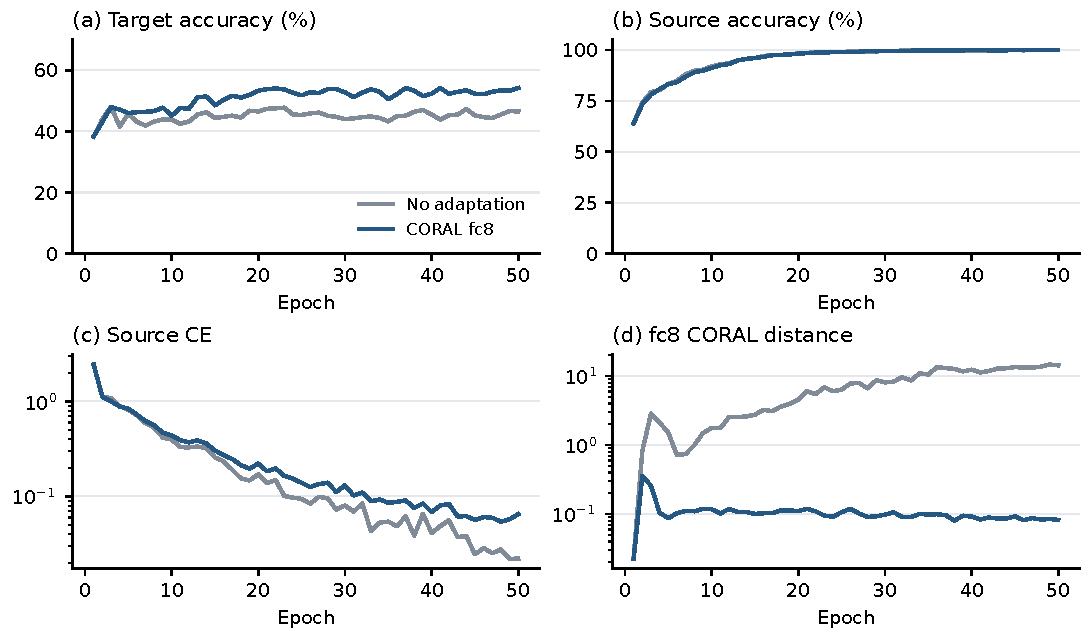
\includegraphics[width=\linewidth]{baseline.pdf}
 \caption{AlexNet 基线实验。两组均训练至第 50 轮；(c)(d) 为对数纵轴。无适应组的 CORAL 距离作为监测量记录，不参与该组反向传播。}
 \label{fig:baseline}
\end{figure}

\begin{table}[H]
 \centering\small
 \caption{多层 CORAL 的完整位置比较。准确率单位为 \%；差值为相对 fc8 第 50 轮的百分点差。最佳值来自历史目标评估，作为补充。}
 \label{tab:layers}
 \begin{tabular}{lrrr}
 \toprule
 对齐位置 & 第 50 轮 & 相对 fc8（pp） & 最佳值 / 轮次\\
 \midrule
 \LayersRows
 \bottomrule
 \end{tabular}
\end{table}

表\ref{tab:layers}与图\ref{fig:layers}给出了所有组合。conv5+fc8 达到 55.09\%，相对 fc8 为 $+0.88\pp$；fc7+fc8 为 54.34\%，相对 fc8 为 $+0.13\pp$。其余全连接联合设置没有形成同样的增益：fc6+fc8 为 52.33\%，fc6+fc7+fc8 为 51.82\%，fc6+fc7 为 45.41\%。单独 fc6、fc7 的结果为 44.40\%、45.91\%。增加层数并未带来单调改善。

\begin{figure}[H]
 \centering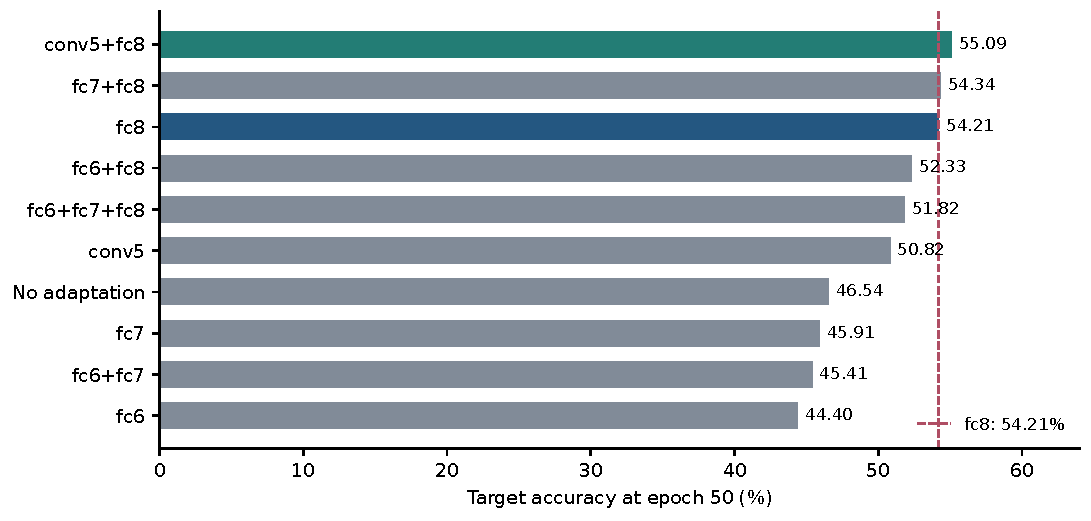
\includegraphics[width=.94\linewidth]{layers.pdf}
 \caption{固定第 50 轮的位置实验。虚线表示 fc8 参照；所有柱均从零起绘制。conv5+fc8 的局部增益与多数多层组合缺少收益这两个事实同时成立。}
 \label{fig:layers}
\end{figure}

\subsection{阶段结论与反思}

\textbf{本阶段没有得到“更多层联合对齐可以有效改善迁移”的结论。}conv5+fc8 提供了 0.88 pp 的正向观察，但这一收益尚没有多种子证据；把它扩展为多层方法的一般优势，会超出当前实验。相反，十组结果说明，对齐位置的选择比层数本身更值得关注。

失败分析首先涉及\textbf{统计估计与任务语义的关系}。batch=128 时，4,096 维图像特征的样本协方差秩至多为 127；全连接层还受到训练态 Dropout 的影响。高维、低秩、带随机扰动的统计量未必稳定刻画需要消除的域变化。fc8 对齐直接作用于类别输出，conv5 则使用另一种局部通道统计，两者可能形成互补。这些是与结构和结果一致的解释，实验没有单独改变 batch、Dropout 或估计器，尚不能识别其中哪项构成主要原因。

另一个关键是\textbf{层位置与层权重发生了联动}。式\eqref{eq:multi}在增加一层时，同时降低已有层的系数；例如 fc8 从单层的 0.5 变为双层的 0.25。因此，联合组与单层组比较的是完整配置，并非“保持 fc8 不变后再加一项”的纯消融。若后续检验层间互补，应固定已有层系数，再单独扫描新增层；还应记录逐层梯度的范数和方向，而非根据不同维度下的原始 CORAL 数值排名。

这一阶段保留的工作参照是固定权重的 fc8 与 conv5+fc8。随后的问题转向：如果固定的总系数没有在训练全过程维持合适的优化关系，能否由训练信号自动学习它？
